\documentclass{article}
\usepackage{/Users/jay/LaTeX/cs}
\usepackage{/Users/jay/LaTeX/matlab}

\newcommand{\hmwkClass}{Digital Image Processing, Spring 2018}
\newcommand{\hmwkTitle}{Homework 4}
\newcommand{\hmwkDueDate}{May 30, 2018}
\newcommand{\tb}{\textbf}

\begin{document}

\thispagestyle{empty}
\section*{\hmwkClass \\
    \normalsize{\hmwkTitle} \\
    \normalsize{DUE DATE: \hmwkDueDate}
}

\hfill{Student ID: B03902129 \, Department: CSIE \, Name: Peng-Yu Chen}

% ------ %
% README %
% ------ %
\subsection*{README}

To run my program, simply type \tb{README} in the Command Window of MATLAB application, then it'll run all .m files and output the .raw images.

\begin{lstlisting}[caption = {README.m}]
    % DIP Homework Assignment #4
    % May 30, 2018
    % Name: Jay Chen
    % ID #: B03902129 
    % email: b03902129@ntu.edu.tw
    
    %#########################################################################
    % Add path first
    %#########################################################################
    
    disp('Add path "./prob1"');
    addpath('./prob1');
    addpath('./readwriter');
    
    % disp('Make a parent folder "./outputs"');
    % mkdir . outputs
    
    %######################################################################### 
    % Problem 1: Optical Character Recognition (OCR)                                           
    % Implementation: Using training set to perform OCR on given images
    %#########################################################################
    
    fprintf('----------------------------------------\n');
    fprintf('Running "prob1"\n----------------------------------------\n');
    prob1();    
\end{lstlisting}

\newpage
% ----------------------------------- %
% PROBLEM 1: Morphological Processing %
% ----------------------------------- %
\subsection*{PROBLEM 1: Optical Character Recognition (OCR)}

In this assignment, I used the method mentioned in the paper - \href{http://ijcsit.com/docs/Volume\%205/vol5issue02/ijcsit20140502254.pdf}{Optical Character Recognition Implementation Using Pattern Matching}. \\

The flowchart of the algorithm: \\

\tikzstyle{block} = [rectangle, draw, text width=10em, text centered, rounded corners, minimum height=2em]
\tikzstyle{line} = [draw, -latex']
\begin{center}
\begin{tikzpicture}[node distance = 1.2cm, auto]
    % Place nodes
    \node [block] (a) {Read training set};
    \node [block, below of=a] (b) {Gray scale conversion};
    \node [block, below of=b] (c) {Feature extraction};
    \node [block, below of=c] (d) {Recognition pattern};
    \node [block, below of=d] (e) {Recognition output};
    % Draw edges
    \path [line] (a) -- (b);
    \path [line] (b) -- (c);
    \path [line] (c) -- (d);
    \path [line] (d) -- (e);
\end{tikzpicture}
\end{center}

First, I extract the features of TrainingSet.raw into 70 binary images sizes of $15 \times 15$.

\begin{figure}[!htb]
    \centering
    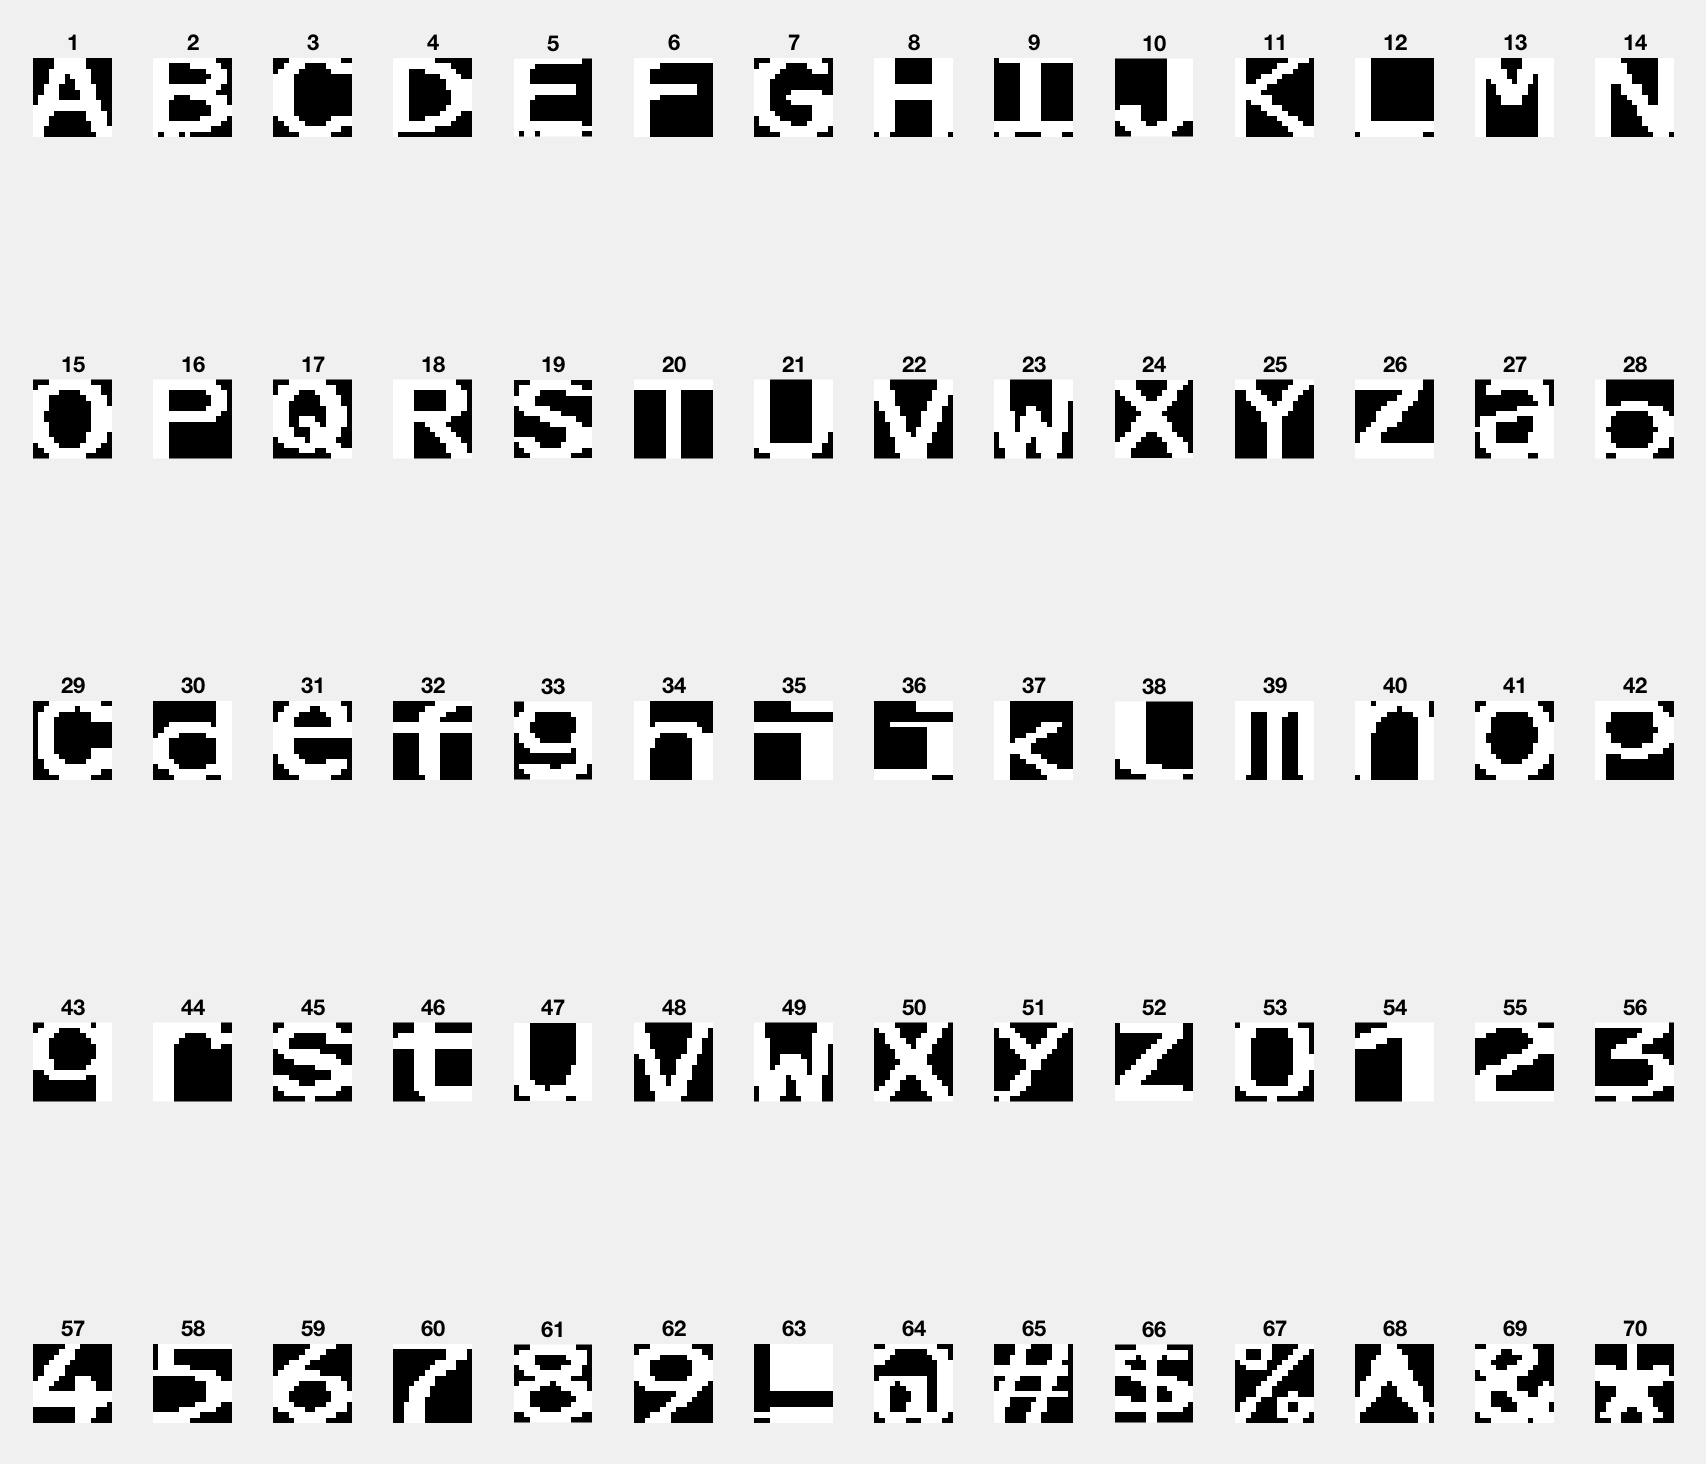
\includegraphics[width=0.8\textwidth]{img/chars.png}
    \caption{Characters of TrainingSet.raw}
\end{figure}

Both sample1.raw and sample2.raw will run the following algorithm except that I perform a Cross Median Filter on sample2.raw first since there are pepper \& salt noises in sample2.raw.

\subsubsection*{Algorithm}
\begin{enumerate}
    \item Label the input image by connected component algorithm implemented in Homework 3.
    \item Get characters of the image.
    \item Extract features of the image.
    \item Reconize the characters based on the RMSE between the feature of the image and the features of TrainingSet.raw.
    \item Output the resulting characters.
\end{enumerate}

Here I want to detail the step of feature extraction. In the following figure, we can see that the binary image has been divided into 5 tracks and each track subdivided into 8 sectors. So we have to calculate number of pixels in each region. (There are $5 \times 8 = 40$ regions.)

\begin{figure}[!htb]
    \centering
    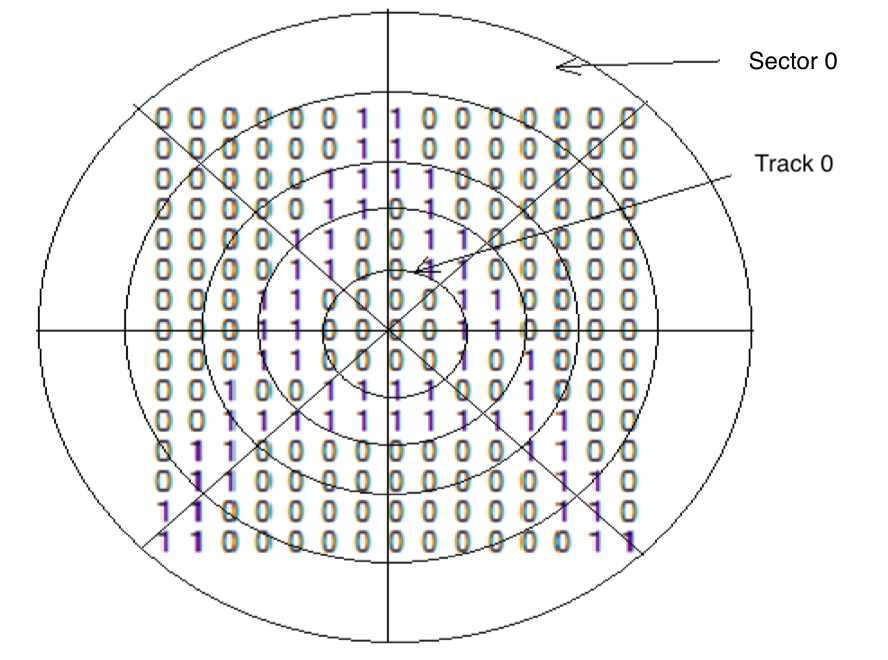
\includegraphics[width=0.5\textwidth]{img/circle.png}
    \caption{Division into tracks and sectors}
\end{figure}

\begin{enumerate}
    \item Identify the center of the binary image. (Here the center is $I(8, 8)$ since the iamge size is $15 \times 15$.)
    \item Calculate radius by finding pixel with maximum
    distance from center using distance formula.
    $$d(point, center) = \sqrt{(x_2 - x_1)^2 + (y_2 - y_1)^2}.$$
    \item Perform $(rad \div 5)$ to identify size of each imaginary track.
    \item Identify 8 imaginary sectors.
    \item Calculate number of 255 (white point) in each region.
\end{enumerate}

I identify the desired character by calculating the RMSE (Root Mean Square Error) between the feature of the image ($I$) and the features ($trainingFeature$) of TrainingSet.raw. Here $c = 1, 2, \dots, 70$ represent 70 characters in the TrainingSet.raw:

$$arg \min_c \sum_{n = 1}^{40} (I^n - trainingFeature_c^n)^2.$$

Finally, I can obtain the output string 'HigX8' and 'SB4T7I'.

\end{document}